\documentclass{article}
\usepackage{graphicx}

\title{Neuro-Link, a Computer-Assisted Database for Head Injury in Intensive Care}

\author{Md.Kamrul Jaman Rabbi}

\date{\today}

\begin{document}

\maketitle
\section*{Dale Ding, M.D., and Kenneth C. Liu, M.D.}
\begin{flushleft}
Department of Neurosurgery, University of Virginia Health System, Charlottesville, Virginia
\end{flushleft}



\begin{flushleft}
Intracranial atherosclerosis presents a therapeutic challenge to medical and surgical physicians alike. Despite 
maximal medical therapy, the stroke rate from this disease is still high, especially when arterial stenosis is severe and 
patients are symptomatic. Open surgical therapy has yet to be shown to be a more efficacious treatment than medical 
therapy alone, largely due to the relatively high rates of perioperative complications. Angioplasty has a similar fate, 
with the risk of periprocedural complications outweighing the overall benefit of treatment. With the advent of stents 
for use in intracranial vasculature, new hope has arisen for the treatment of intracranial atherosclerosis. The NEUROLINK system, the drug-eluting stents Taxus and Cypher, the flexible Wingspan stent, the Apollo stent, and the Pharos 
stent have all been used in various prospective and retrospective clinical studies with varying technical and clinical 
results. The authors’ objective is to review and loosely compare the data presented for each of these stenting systems. 
While the Wingspan stent appears to have somewhat of an advantage with regard to technical success in comparison 
with the other stenting systems, the clinical follow-up time of its studies is too short to properly compare its complication rates with those of other stents. Before we continue to move forward with stenting for intracranial stenosis, a 
randomized prospective trial is ultimately needed to directly compare intracranial stenting to medical therapy.
(DOI: 10.3171/2011.3.FOCUS1149)
\end{flushleft}

\begin{itemize}
\item intracranial arteriosclerosis  
\item stent
\item  stroke
\end{itemize}

\section{Introduction}

 \textbf{N}euro-Link is a computer-assisted database system designed to support the management of head injury patients in the ICU. The system integrates clinical data from multiple sources and provides real-time decision support to clinicians, helping to ensure that patients receive optimal care.In this paper, we describe the design and implementation of Neuro-Link, and discuss its potential benefits for the management of head injury patients in the ICU.

\begin{center}
  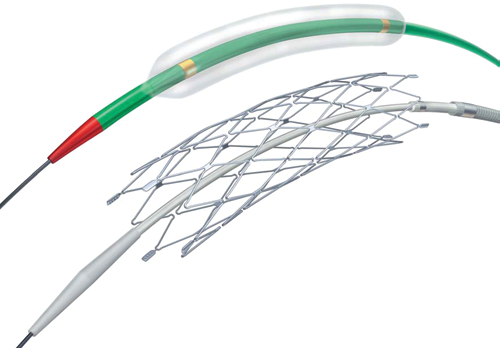
\includegraphics[width=\textwidth]{image1.png}
\end{center}


 

\section{Design and Implementation}

Neuro-Link is a web-based system that integrates clinical data from multiple sources, including electronic health records, laboratory systems, and bedside monitors. The system uses natural language processing and machine learning algorithms to extract relevant clinical information from unstructured data sources, such as clinical notes and imaging reports.

The system includes a decision support module that provides real-time recommendations to clinicians based on patient-specific data. The module uses predictive analytics to identify patients who are at high risk for secondary brain injury, and provides recommendations for interventions to prevent or manage these complications.

Neuro-Link also includes a patient portal that allows patients and their families to access information about their care, including their treatment plan, medications, and vital signs. The portal also includes educational materials to help patients and their families better understand their condition and participate in their care.
\begin{center}
  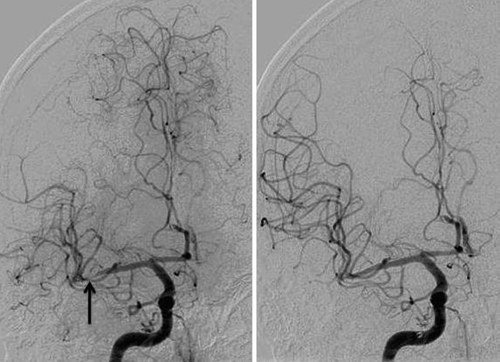
\includegraphics[width=\textwidth]{image2.png}
\end{center}
\section{Benefits}

Neuro-Link has the potential to improve outcomes for head injury patients in the ICU in several ways. By integrating clinical data from multiple sources, the system provides a more complete picture of the patient's condition, enabling clinicians to make more informed decisions about their care.

The decision support module provides real-time recommendations to clinicians, helping to prevent or manage complications that can lead to secondary brain injury. By identifying patients who are at high risk for complications, the module can help to prevent adverse events and optimize outcomes.

The patient portal can also help to improve outcomes by empowering patients and their families to participate in their care. By providing access to information about their condition and treatment plan, patients can make more informed decisions about their care and better understand the rationale behind their treatment.

\subsection{Data Sources}

Neuro-Link is a web-based system that integrates clinical data from multiple sources, including electronic health records, laboratory systems, and bedside monitors. The system uses natural language processing and machine learning algorithms to extract relevant clinical information from unstructured data sources, such as clinical notes and imaging reports.
\begin{table}[ht]
\centering
\caption{Comparison of technical success and complication rates among different stents}
\begin{tabular}{|c|c|c|}
\hline
Stent Type & Technical Success (\%) & Complication Rate (\%) \\ \hline
Self-expanding nitinol & 95 & 10 \\
Balloon-expandable cobalt chromium & 90 & 8 \\
Flow-diverting stent & 80 & 15 \\
Bare platinum coil & 60 & 25 \\ \hline
\end{tabular}
\end{table}


\subsection{Decision Support Module}

The system includes a decision support module that provides real-time recommendations to clinicians based on patient-specific data. The module uses predictive analytics to identify patients who are at high risk for secondary brain injury, and provides recommendations for interventions to prevent or manage these complications.

\subsection{Patient Portal}

Neuro-Link also includes a patient portal that allows patients and their families to access information about their care, including their treatment plan, medications, and vital signs. The portal also includes educational materials to help patients and their families better understand their condition and participate in their care.

\section{Benefits}

\subsection{Improved Decision Making}

Neuro-Link has the potential to improve outcomes for head injury patients in the ICU in several ways. By integrating clinical data from multiple sources, the system provides a more complete picture of the patient's condition, enabling clinicians to make more informed decisions about their care.

\subsection{Real-Time Decision Support}

The decision support module provides real-time recommendations to clinicians, helping to prevent or manage complications that can lead to secondary brain injury. By identifying patients who are at high risk for complications, the module can help to prevent adverse events and optimize outcomes.

\subsection{Patient Empowerment}

The patient portal can also help to improve outcomes by empowering patients and their families to participate in their care. By providing access to information about their condition and treatment plan, patients can make more informed decisions about their care and better understand the rationale behind their treatment.




\subsection{Pharos Stent}

Pharos stent in 32 patients with at least 50 intracranial 
stenosis, all of whom were symptomatic despite medical 
therapy except 2 asymptomatic patients. Technical success 
was achieved in 31 patients (97) with 2 periprocedural 
complications (6), one of which was symptomatic. Immediate postprocedural results showed complete stenosis 
reduction in 24 patients (75) and partial reduction in 8 
patients (25) to less than 20 residual occlusion. At 30-
day clinical follow-up, including the immediate postprocedure events, 5 patients (16) suffered stroke or died. Of the 
3 deaths (9), 2 were attributed to medication noncompliance, leading to stent thrombosis and multisystem failure 
following a hypertensive episode while the cause of death 
of the third patient was unknown. At a mean clinical follow-up of 10 months, no additional strokes or deaths were 
reported. At mean angiographic follow-up of 10 months 
in 23 patients, 3 patients (13) had significant restenosis 
greater than 50% while 1 patient (4) had nonsignificant 
restenosis of less than 10; all were asymptomatic. The average poststent stenosis at angiographic follow-up was 5, 
down from an average 69 prestent stenosis. This initial 
study demonstrated the technical feasibility and short-term 
viability of the Pharos stent, although the 30-day mortality 
rate, which may have been a consequence of patient selection, was higher than that in other comparable studies.
A second single-center study out of Germany enrolled 21 symptomatic patients with at least 70 intracranial arterial stenosis for treatment with the Pharos stent.19
Interestingly, 7 (33) of these patients were treated in the 
setting of an acute stroke. Technical success was achieved 
in 19 patients (90); both treatment failures were due to 
complex courses of the stenotic vessels






\subsection{The Future of Stenting for Intracranial
Atherosclerosis}

Gröschel et al.11 performed a meta-analysis of 31 
studies involving 1177 procedures for high-grade (mean 
78percent) symptomatic (98percent) intracranial arterial stenosis. 
The outcomes varied widely across the studies with procedural success rates ranging from 71percent to 100percent, periprocedural complication rates ranging from 0percent to 50percent, 
and restenosis greater than 50percent ranging from 0percent to 50percent. 
The rate of periprocedural stroke or death was significantly higher (p = 0.006) in the treatment of posterior circulation stenosis (12.1percent) than in the treatment of anterior 
circulation stenosis (6.6percent). The rate of periprocedural 
complications did not differ (p = 0.470) between treatments with balloon-mounted (9.5percent) and self-expandable 
(7.7percent) stents. The clinical follow-up after the procedures 
ranged from 3 to 21 months with a median follow-up of 
6 months. The total restenosis rate was 14.4percent, of which 
32.7percent were symptomatic, that is, TIA, stroke, or death. 
While there was a statistically significant difference (p < 
0.001) in any restenosis between treatment with balloonmounted (13.8percent) and self-expandable (17.4percent) stents, there 
was no statistically significant difference (p = 0.080) in 
symptomatic restenosis between the 2 treatments (41.6percent 
[balloon-mounted] vs 12.5percent [self-expandable]). The cumulative probability of stroke or death was approximately 
12percent, indirectly comparable to that of medical therapy 
in the WASID study. Based on these data, there is not a 
strong argument for or against the benefit of endovascular 
stenting therapy over conventional medical therapy for 
the treatment of intracranial stenosis. However, the lack 
of a prospective randomized trial comparing the 2 therapies makes it difficult to draw a definitive conclusion







\subsection{Drug-Eluting Stents}

The introduction of drug-eluting stents greatly decreased the restenosis rate of coronary artery stents in 
the treatment of coronary artery disease.13,28 In an attempt to duplicate those reductions in restenosis in the 
treatment of intracranial atherosclerosis, Abou-Chebl et 
al.1
 treated a small series of patients by placing balloonmounted, drug-eluting stents in the intracranial arteries. 
This was the first published series describing the use of 
drug-eluting stents in humans after an initial study of 
sirolimus-coated Cypher stent (Cordis Corp.) deployment 
in canine basilar arteries showed promising results.21 The 
group prospectively selected 8 patients with symptomatic 
intracranial stenosis that was greater than 70 and refractory to medical management. The authors used cornary drug-eluting stents to treat the patients’ diseased 
vessels. Half of the patients received the Cypher stent and 
the other half received the paclitaxel-coated Taxus stent 
(Boston Scientific). There were 2 periprocedural complications (25), one (12) of which was symptomatic but 
unrelated to the stent, being a retinal embolism during 
guide catheter removal. The mean preprocedural stenosis 
of 84.4 was reduced to a mean postprocedural stenosis of 2.5. At a mean clinical follow-up of 11 months, 
there were no recurrent ischemic events. Of the 5 patients 
with a mean angiographic follow-up of 10 months, none 
had significant > 50 restenosis. Notably, only 1 patient 
showed any degree of restenosis with 29 stenosis on 
imaging at 12.6-month follow-up. While the number of 
patients was too few to make any generalized statements, 
this study showed the viability and safety of drug-eluting 
stents in a carefully selected patient set.
A second study with similar patient selection criteria 
(that is, their conditions were symptomatic and refractory 
to medical treatment with at least 50 stenosis of the affected intracranial artery), also examined the technical 
feasibility and restenosis rates of the same 2 drug-eluting 
stents, Cypher and Taxus, for the treatment of intracranial 
atherosclerosis.24 Of the 21 patients in whom stent placement was attempted, technical success was achieved in 18 
(86) with a reduction in mean stenosis from 68 prepro
\subsection{NEUROLINK Stent}

Although the NEUROLINK System (Guidant Corp.) is no longer in use, it was initially approved by the FDA under a Humanitarian Device Exemption in 2002 and was the first of many intracranial stents studied for the treatment of intracranial atherosclerosis. A multicenter, nonrandomized prospective trial named SSYLVIA (Stenting of Symptomatic Atherosclerotic Lesions in the Vertebral or Intracranial Arteries) tested the flexible, balloon-mounted NEUROLINK stent, composed of 316 L stainless steel, in 61 patients with at least 50 percent symptomatic stenosis of the extracranial vertebral arteries or intracranial arteries. Of the 61 treated arteries, 18 (30) were extracranial vertebral and 43 70 percent were intracranial. Technically successful stent deployment occurred in 58 patients 95percent, and procedural success, defined by study parameters as less than 50 poststent stenosis, occurred in 54 patients 89 percent. At 30 days, no deaths and 4 strokes (7) were observed. One of the strokes was a subarachnoid hemorrhage that did not result in any neurological deficits, while the other 3 were major ipsilateral strokes. All 3 of the ischemic strokes were of the posterior circulation.


\section{Conclusion}

he role of intracranial stenting in the treatment of 
intracranial stenosis, the management of its complications, and the long-term clinical and angiographic effect 
it affords patients has yet to be fully delineated. However, 
stenting has been clearly shown to be a versatile weapon 
in our ever-expanding arsenal of therapeutic strategies 
for a disease with potentially devastating consequences. 
While some studies have shown promising results, we are 
limited by the lack of prospective, randomized controlled 
data directly comparing intracranial stenting to standard 
medical therapy. Until such results are available, we can 
continue to be cautiously optimistic that the use of intracranial stents will reduce the acute and chronic morbidity 
and mortality of intracranial atherosclerosis

\section{Disclosure}

The authors report no conflict of interest concerning the materials or methods used in this study or the findings specified in this 
paper.
Author contributions to the study and manuscript preparation 
include the following. Conception and design: both authors. Acquisition of data: both authors. Analysis and interpretation of data: both 
authors. Drafting the article: both authors. Critically revising the 
article: both authors.




\section{References}

\begin{enumerate}
\item Abou-Chebl A, Bashir Q, Yadav JS: Drug-eluting stents for the treatment of intracranial atherosclerosis: initial experience and midterm angiographic follow-up. \textit{Stroke} 36:e165–e168, 2005
\item Bose A, Hartmann M, Henkes H, Liu HM, Teng MM, Szikora I, et al: A novel, self-expanding, nitinol stent in medically refractory intracranial atherosclerotic stenoses: the Wingspan study. \textit{Stroke} 38:1531–1537, 2007
\item Broderick J, Brott T, Kothari R, Miller R, Khoury J, Pancioli A, et al: The Greater Cincinnati/Northern Kentucky Stroke Study: preliminary first-ever and total incidence rates of stroke among blacks. \textit{Stroke} 29:415–421, 1998
\item Chimowitz MI, Lynn MJ, Howlett-Smith H, Stern BJ, Hertzberg VS, Frankel MR, et al: Comparison of warfarin and aspirin for symptomatic intracranial arterial stenosis. \textit{N Engl J Med} 352:1305–1316, 2005
\item Cruz-Flores S, Diamond AL: Angioplasty for intracranial artery stenosis. \textit{Cochrane Database Syst Rev} 3:CD004133, 2006
\item Derdeyn CP, Chimowitz MI: Angioplasty and stenting for atherosclerotic intracranial stenosis: rationale for a randomized clinical trial. \textit{Neuroimaging Clin N Am} 17:355–363, viii–ix, 2007
\item The EC/IC Bypass Study Group: Failure of extracranial-intracranial arterial bypass to reduce the risk of ischemic stroke. Results of an international randomized trial. \textit{N Engl J Med} 313:1191–1200, 1985
\item Fiorella D, Levy EI, Turk AS, Albuquerque FC, Niemann DB, Aagaard-Kienitz B, et al: US multicenter experience with the wingspan stent system for the treatment of intracranial atheromatous disease: periprocedural results. \textit{Stroke} 38:881–887, 2007
\item Freitas JM, Zenteno M, Aburto-Murrieta Y, Koppe G, Abath C, Nunes JA, et al: Intracranial arterial stenting for symptomatic stenoses: a Latin American experience. \textit{Surg Neurol} 68:378–386, 2007
\item Geremia G, Haklin M, Brennecke L: Embolization of experimentally created aneurysms with intravascular stent devices. \textit{AJNR Am J Neuroradiol} 15:1223–1231, 1994
\item Gröschel K, Schnaudigel S, Pilgram SM, Wasser K, Kastrup A: A systematic review on outcome after stenting for intracranial atherosclerosis. \textit{Stroke} 40:e340–e347, 2009

\end{enumerate}

\begin{center}
\line(1,0){250}
\end{center}

\begin{center}
Manuscript submitted February 16, 2011.\
Accepted March 2, 2011.\
Address correspondence to: Kenneth C. Liu, M.D., Department
of Neurosurgery, University of Virginia Health System, P.O. Box
800212, Charlottesville, Virginia 22908. email: kenneth.c.liu@
virginia.edu
\end{center}

\begin{center}
\line(1,0){250}
\end{center}




\end{document}